In this chapter, we focus on \emph{Pac-Man} as learning environment and on our collection of agent programs based on deep Q-learning.

The project itself consists of a light framework for training, running and evaluating RL agents.
Our framework is compatible with various other environments, as long as they respect the interface provided by OpenAI Gym.
The feature set includes automatic checkpoints, cloud-friendly deployment and a performance analysis toolkit.

In Section \ref{section:modelling-the-problem}, we justify why we choose to study the game of \emph{Pac-Man} and formalize the specifications of it as a learning environment.

In Section \ref{section:approach-algorithms}, we introduce some of the algorithms built into our collection of autonomous agents.
The main method is vanilla DQN, which was covered previously in Section \ref{section:dqn}.
However, in this section, we present two important improvements over it -- double DQN and Prioritized Experience Replay.

In Section \ref{section:implementation}, we take a look at each subcomponent of an individual agent program and map each one to notions from our previous chapter.
Each agent has its own module and inherits a specific structure from a prototype.

In Section \ref{section:technologies}, we present a rundown of our technology stack, whose core is the Python programming language. The framework is built on the PyTorch machine learning library but makes use of many other ML and data science libraries.

We wrap up this chapter with Section \ref{section:user-manual} which consists of a short instruction manual for users to start local or remote training sessions, use the provided performance measurement tools and extend the existing collection of agents.

\clearpage

\section{Modelling the Problem} \label{section:modelling-the-problem}
The problem we solve in this thesis is three-fold.
Firstly, we specify a variant of a task environment for \emph{Pac-Man}, defining goals and rewards to view it through the lens of reinforcement learning.
Secondly, we train agents to ``solve’’ that environment, i.e. explore and learn to take optimal decisions to achieve the established goals.
And lastly, we compare agents based on proximity to their goals, mean reward and learning stability.

\textbf{\textit{Pac-Man}} is a classic video game developed by Toru Iwatani and published by Namco Ltd. in 1980 \cite{pacman-in-academia}.
The game was originally released as an arcade game and it quickly became the most commercially sucessful arcade game ever created.
The original hit gave rise to a series of ``licensed clones'', which targeted a number of popular platforms, such as the Atari 2600, the Nintendo Entertainment System (NES), the Nintendo GameBoy, etc.
Besides its commercial success, \emph{Pac-Man} has been an appealing object of study for academia, across a number of fields, ranging from psychology to mathematics and computational intelligence \cite{pacman-in-academia}.

\begin{figure}[h]
    \centering
    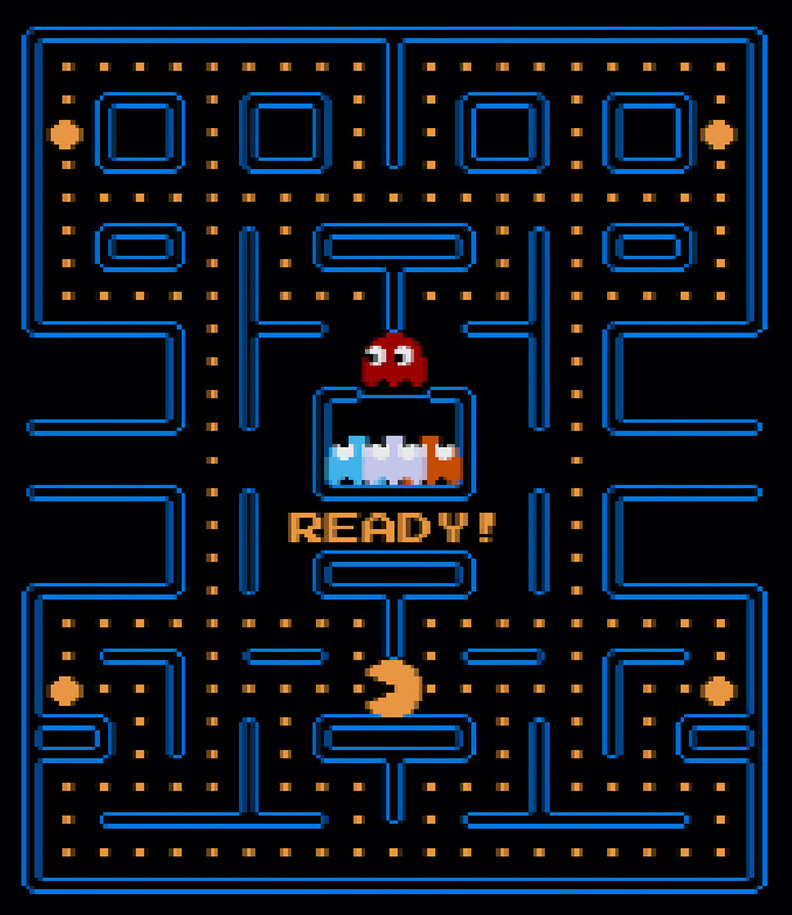
\includegraphics[width=0.4\textwidth]{nes-pac-man.jpg}
    \caption{Screen capture of the starting configuration from Nintendo's NES variant of the game.}
    \label{fig:pac-man-screen}
\end{figure}

The game's mechanics are intuitive but engaging enough to be fun.
It allows simple four-directional movement.
The player is represented as a yellow character with a distinctive circular shape (with a ``missing slice''\footnotemark{} representing its mouth).
\footnotetext{Iwatani's stated inspiration for Pac-Man's design was a pizza with a missing slice. \cite{pacman-gameinformer}}
The board is a bidimensional maze, featuring tunnels which loop around each other, i.e. entering a tunnel on one side will transport the player out through the opposite side of the board.
\textbf{Pellets} (or \emph{dots}) are placed at almost every position, and the goal of every level is to collect all pellets.
Most renditions of the game feature four \textbf{ghosts} which will chase the player around the board.
Collisioning with any of the ghosts results in losing a life and being repositioned to the start (without losing progress on dots).
The ghosts have different ``personalities'' -- each of them has a different approach for chasing Pac-Man.
There are special power pellets in each of the four corners (seen in Figure \ref{fig:pac-man-screen}).
\textbf{Power pellets} grant Pac-Man temporary immunity from ghosts and changes the power dynamic in the game for a short time: the ghosts enter \textbf{``scared'' mode} and reverse their direction to run away.
In this mode, the player gets an increasing score for every ghost it eats.

\emph{Pac-Man} can be defined as a 2D gridworld environment, where exploration is necessary to reach the goal.
This class of task environments is common throughout RL literature and has some common properties:
\begin{itemize}
    \item they have discrete bidimensional representation;
    \item an agent has a finite set of options at every time step.
\end{itemize}

\textbf{Gridwords} are used in literature to clearly define and \textbf{isolate} agent goals.
A simplistic environment with a clear task is also beneficial for agent learning due to its low degree of environmental noise -- the agent can ``focus'' on the task.
The ease of customizability of the rules inside a gridworld allows creating interesting strategy games to test agents’ decision-making capabilities.
New non-trivial grid-based environments are an area of open research -- for example, the \emph{Pommerman} benchmark \cite{pommerman-paper} has been formulated as a novel interesting multi-agent problem which does not yet have an optimal solution.

\emph{Pac-Man} has a few advantages which make it interesting to study from a RL perspective.

First of all, it provides a \textbf{shaped reward} built-into the game mechanics.
In reinforcement learning, a \textbf{sparse reward} is a large reward which is delayed for a relatively large number of steps.
A sparse reward would be, for example, if we would only reward the agent at the end of the game.
Shaped rewards, in contrast, equate with providing gradual feedback to the agent.
This can improve learning and lead to better outcomes earlier in training, as good behaviours become immediately obvious to the agent.

In \emph{Pac-Man}, the pellets, placed uniformly over the board, provide a shaped reward which directly reflects the goal of the game, i.e. to eat all pellets on a board without getting caught.
Moreover, they \textbf{incentivize exploration} as the reward is higher in places the agent has not visited before.

Second of all, \emph{Pac-Man} requires the agent to develop non-trivial strategies.
The game requires balancing two equally important subgoals: fully covering the game board to consume every available pellet, and running away from the chasing ghosts.
This gives rise to complex and potentially problematic situations for the player, which require \textbf{planning}.
This raises an interesting question regarding the potential of existing algorithms to learn \textbf{long-term strategies} similar in performance to human players.

The \textbf{reward function} we use in this thesis for our \emph{Pac-Man} environment is a combination of a few properties of the environment state.
The most important component is the \textbf{score}.
Score changes will determine a proportional reward for the agent.
Significant score increases are provided by eating pellets but a more interesting mechanic is eating ghosts when the player is invincible.
Each ghost eaten will provide a higher reward, thus conditioning the agent to chain as many ``kills'' as possible.
Typical of arcade games, the mechanics are built such that the score can \emph{only increase} over time.
This creates a necessity to \emph{counterbalance} by finding opportunities for \textbf{punishment}.
We choose to strongly penalize the agent for losing a life.
There are other possible candidates for ``punishment'' events, but we consider ``death on ghost contact'' to be the most important for capturing the goal of the game.

\section{Algorithms} \label{section:approach-algorithms}
In this section, we present the main algorithms powering the autonomous agents evaluated in this thesis. In our collection, \textbf{vanilla DQN} serves both as a stand-alone implementation, as well as a fundamental building block of more advanced algorithms.
The original DQN, however, is already covered by Section \ref{section:dqn} of our theory chapter and we will omit it here for conciseness.
Instead, this section deals with \textbf{double DQN} and \textbf{prioritized experience replay (PER)}, both of which address shortcomings of the original algorithm.

\subsection{Double Q-learning} \label{section:double-dqn}
Double DQN \cite{ddqn-paper} is an algorithm in the deep Q-learning family, discovered and published by DeepMind researcher Hado van Hasselt along with several other colleagues.
The study determines that general Q-learning (and, by extension, deep Q-learning) suffers from a problem known as a \textbf{maximization bias} and adapts the original algorithm to account for this and counteract the bias.

Stated simply, a \textbf{maximization bias} is an implicit preference of the algorithm to overestimate values, despite divergence from the true value.
Some control algorithms, such as Q-learning, fundamentally depend on using the maximum over estimated values as an estimate for the maximum value \cite{rlai}.
This leads to situations where noisy reward signals, prevalent in real-world environments, can significantly destabilize learning and slow down training progress.

Hasselt proposes \emph{double learning} to counteract this bias.
This requires two independent approximators of the action-value function -- we will denote them $Q_1$ and $Q_2$.
At every step, the approximators are \emph{intermittently} used either to pick an action or to estimate its value.
The paper proves that this decoupling is sufficient to accomplish an unbiased estimation.
Which function serves which role can be chosen uniformly at random at every learning step at practically no cost.
Equation \ref{eqn:double-learning-rule} states the double learning \textbf{update rule}, considering the situation in which $Q_1$ picks the action (and is updated) while $Q_2$ gives the estimate which we bootstrap from.

\begin{equation} \label{eqn:double-learning-rule}
\begin{aligned}
Q_1(S_t, A_t) & \leftarrow Q_1(S_t, A_t) \\
    & + \alpha [ R_{t+1} + \gamma Q_2(S_{t+1}, \argmax_{a \in A} Q_1(S_{t+1}, a)) - Q_1(S_t, A_t)]
\end{aligned}
\end{equation}

A drawback of the double learning algorithm is that it requires double the amount of memory of the original. 
Despite this, it still performs one update per step, so the running time is equivalent to that of its predecessor.
% to steal more content space, include and explain the example from RLAI

\subsection{Prioritized Experience Replay (PER)} \label{section:per}
\textbf{Prioritized experience replay} (often shortened as \emph{PER}) is an extension of deep Q-learning, also developed by a team at DeepMind, led by Tom Schaul \cite{per-paper}.
The paper focuses on improving experience replay from classic DQN.

Recall from Section \ref{section:dqn} the principle of \textbf{experience replay}, which consists of storing all transitions the agent experiences in order to revisit them later during training.
Reusing experiences over multiple update steps reduces the number of samples required for learning.
The original approach suggests that the experiences are revisited by sampling them uniformly at random from the replay memory.
This has the important role of \emph{decoupling} experiences -- which in the case of successive video game frames, are by nature highly correlated -- to avoid introducing \emph{high variance} into the system (which can cause overfitting).

The foundational hypothesis of the paper at \cite{per-paper} is that some transitions have higher ``teaching’’ potential than others.
The \emph{prioritization} mentioned in the title refers to finding an ordering over experiences which properly reflects this potential.
The authors chose \emph{absolute TD-error} as a good approximation for utility in learning -- for several reasons.
Firstly, since larger errors suggests that a prediction is further from the agent’s current expectations, minimizing larger errors would naturally improve performance the most.
This supposition has intuitive appeal because \textbf{humans} likewise learn proportionally more from experiences that contradict their existing beliefs the most.
Additionally, TD-error is already computed as part of the normal update cycle in DQN so extending the implementation to PER does not require significant overhaul of the algorithm.

The paper develops two separate models for prioritizing experience based on error.
Each model specifies how priorities are computed and stored.

\textbf{Rank-based prioritization} involves keeping track of the rank each transition occupies.
Each transition would thus have an assigned priority of $p = 1 / rank$.
This requires an additional data structure, capable of online sorting, such as a heap, as some ranks will change at every update step.

Since the replay memory can potentially store millions of transitions, \textbf{optimization} is necessary to prevent severely hindering performance.
Changing every rank at every update step is impractical and would outweigh the benefits of prioritization.
In order to mitigate this, the authors propose to only re-evaluate the ranks of transitions in the sampled mini-batch.
This \textbf{``lazy’’ approach} retains its desirable properties of learning more efficiently than DQN while not adding an insane amount of computation.

\textbf{Proportional prioritization} simply assigns a priority equal to the absolute TD-error plus an $\epsilon$: $p_{i} = |\delta_{i}| + \epsilon$.
The $\epsilon$ (which should not be confused with our exploration coefficient in $\epsilon$-greedy) is an offset keeping all priorities above $0$.

The second part of the algorithm is common to both models and consists of actually assigning probabilities based on priority and building the distribution over the transitions. The formula in (\ref{eqn:per-probability}) gives an outline of the method.

\begin{equation} \label{eqn:per-probability}
    P(i) =  \left( \frac{p_i}{\sum_{k}{p_{k}}} \right)^\alpha
\end{equation}

The $\alpha$ parameter in this equation represents the degree of prioritization, i.e. a higher $\alpha$ will determine a larger difference between the probabilities of any two consecutive transitions (when ordered by priority).

To sample according to the obtained distribuition, a sum tree is used.
A \textbf{sum tree} is a specialized type of segment tree -- a tree data structure which stores \emph{statistics} (e.g. minimum, maximum, sum etc.) of its leaf nodes.
The values of the leaf nodes are usually stored in an array.
The structure is designed to compute interval queries over that array, such as the sum of all values between indices $x$ an $y$, in $\mathcal{O}(\log{n})$, while also allowing fast updates to the underlying data.

\section{Implementation} \label{section:implementation}
The models and algorithms presented throughout our theory chapter and in the previous section are incorporated into our framework and implemented using Python and the PyTorch machine learning library.
The framework is divided into several modules which we detail below.

The \verb|common| package contains classes which are shared among all agent implementations, including those concerning training and evaluation, but also configuration, and a checkpoint manager.

Each agent implementation has its own package: \verb|deepq| is the vanilla DQN agent, \verb|per| implements prioritized experience replay on top of the default DQN, and \verb|doubledqn| and \verb|doubleper| are the double Q-learning versions of the former two.
We cover them in Section \ref{section:agent-modules}.

The \verb|replay_memory| package contains the logic used for memorizing transitions (units of agent experience).
This package is used by all agents to store, sample and replay transitions.
We are keeping it isolated because it is clearly logically separate and because it is complex on its own.

\verb|ds| is short for ``data structures'' and contains our implementation of the sum tree required by \verb|replay_memory.PrioritizedReplayMemory|.

The \verb|wrappers| package contains a helper class which works as a layer on top of OpenAI Gym to implement a few missing features required to properly run and test agents according to the original papers.

While not a package per se, but kept separately from our training logic, we have our Jupyter notebooks (in \verb|notebooks|).
We use those to analyze scores, to graph and benchmark agent performance.
Inside this directory is an isolated \verb|plot| package, custom-built to allow us to work with both data gathered from either a single run or from multiple runs of the same configuration -- this logic is encapsulated in the \verb|SingleRunData| and \verb|MultiRunData| classes.

\subsection{\texttt{Trainer} and \texttt{Evaluator}}

\begin{figure}[ht]
    \centering
    \begin{subfigure}[b]{0.5\textwidth}
        \centering
        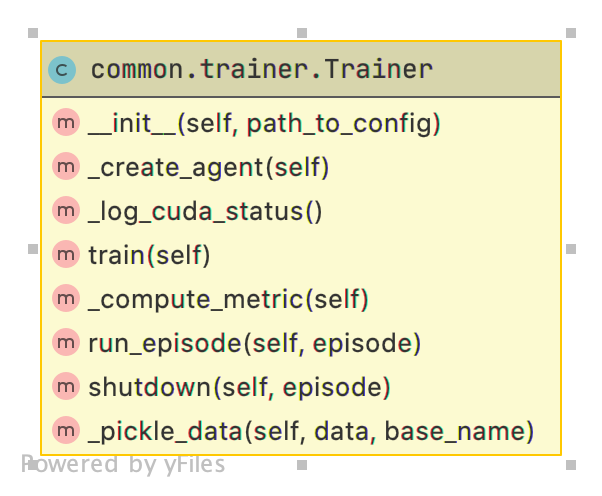
\includegraphics[width=0.5\textwidth]{app-trainer.png}
        \caption{Class diagram of \texttt{Trainer}.}
        \label{fig:trainer-diagram}
    \end{subfigure}%
    \hfill
    \begin{subfigure}[b]{0.5\textwidth}
        \centering
        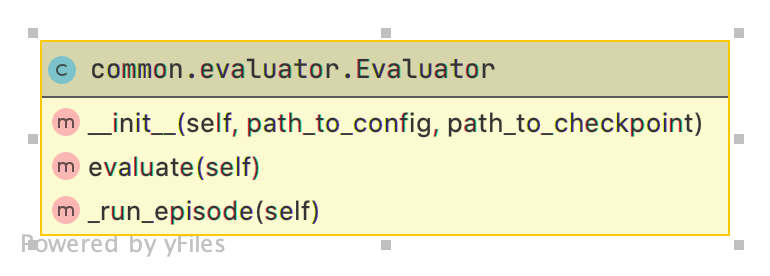
\includegraphics[width=0.5\textwidth]{app-evaluator.png}
        \caption{Class diagram of \texttt{Evaluator}.}
        \label{fig:evaluator-diagram}
    \end{subfigure}
\end{figure}

\texttt{Trainer} and \texttt{Evaluator} host the main loop and constitute (separate) entry points into the system.
The \textbf{trainer} can differ between algorithms and contains more complex procedures overall.
The \textbf{evaluator} is roughly doing the same thing, but is more universal as it does not need to encapsulate any algorithm-specific logic.

Both systems start by loading the configuration file using the \texttt{ConfigLoader}.
This is a simple utility class which loads a \texttt{YAML} file into memory.
After the data is loaded, each level has the responsibility to parse it according to its requirements.
For example, we generally group hyperparameter data under the \texttt{model} category of a configuration file, representing parameters required to calibrate the algorithm.
The trainer's job is \textbf{general} -- to redirect the model parameters to the agent -- and thus does not do any parsing by itself.
It is the agent’s job to parse and validate the data.

For training, we initialize every needed component: agent, environment, checkpoint manager, etc.
The main loop consists of fetching the current state from the emulator, feeding it to the agent for learning and processing, then playing the agent’s chosen action into the emulator.
At every iteration, we log scores, compute statistics for plotting and call the checkpoint manager to check if the current state needs to be saved.
An activity diagram of the training process is provided in Figure \ref{fig:training-loop-activity-diagram}.

\begin{figure}[h]
    \centering
    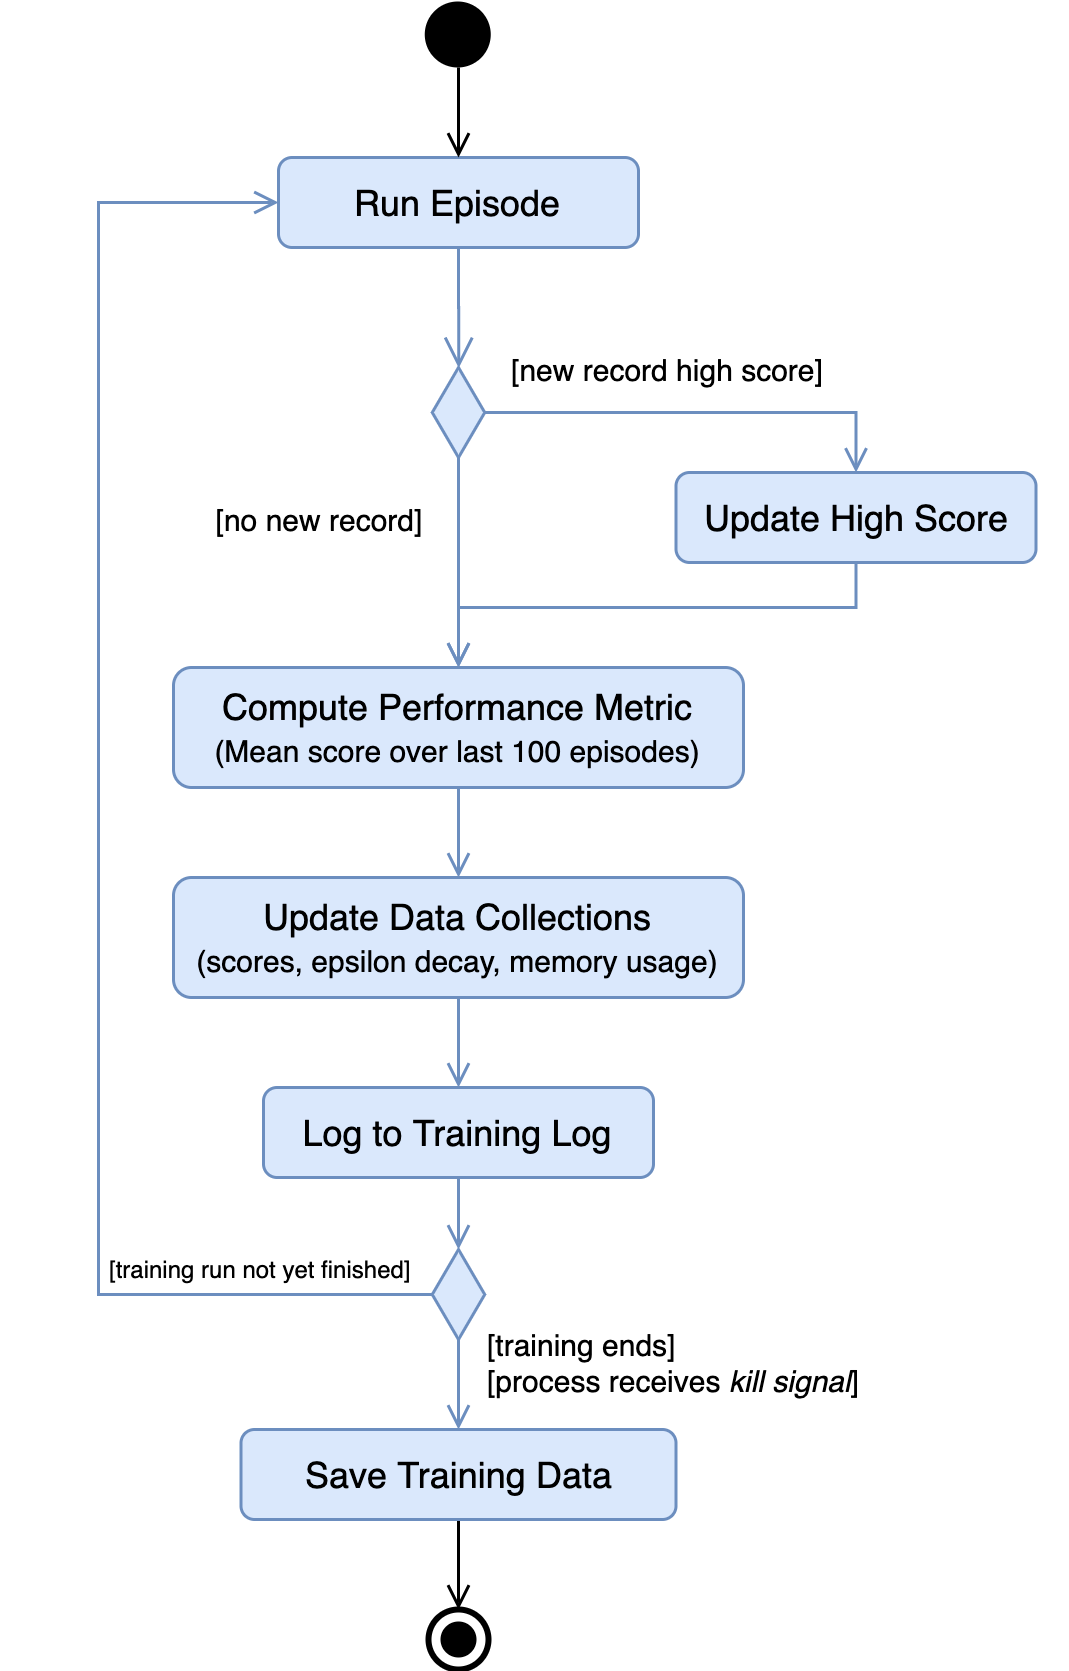
\includegraphics[width=0.6\textwidth]{training_activity_diagram.png}
    \caption{Activity diagram of the main training loop in our \texttt{train()} function.}
    \label{fig:training-loop-activity-diagram}
\end{figure}

\begin{figure}
    \centering
    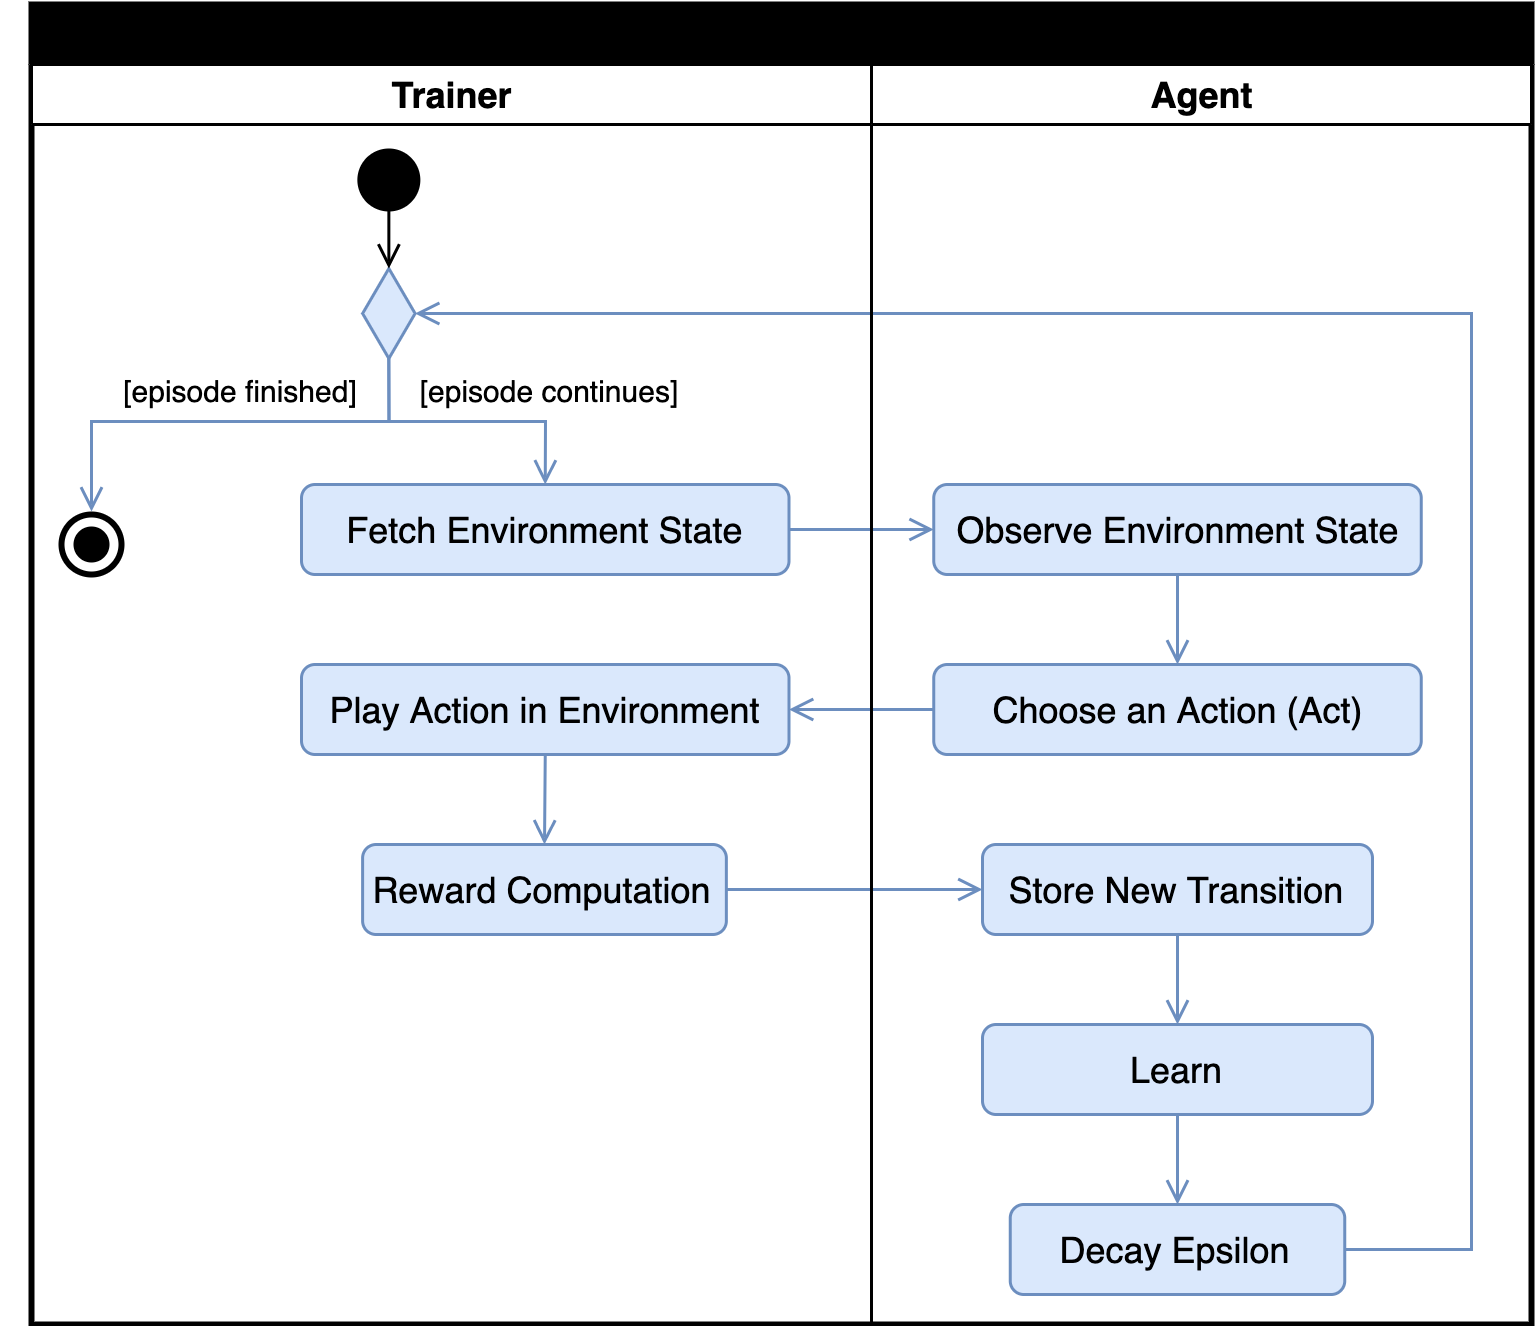
\includegraphics[width=\textwidth]{run_episode_activity_diagram.png}
    \caption{An activity diagram corresponding to the ``Run Episode'' sub-task from Figure \ref{fig:training-loop-activity-diagram}. This diagram highlights the agent-environment loop.}
    \label{fig:run-episode-diagram}
\end{figure}

The \texttt{Trainer} class has a \emph{graceful exit} procedure, the \texttt{shutdown} method.
It is triggered automatically at the end of training and mapped to the \texttt{SIGKILL} signal.
Training jobs are designed to be able to run for a long time inside a cloud instance, including on preemptible instances\footnotemark{}.
\footnotetext{relatively low-cost instances which can be terminated at any time if required by the cloud provider.}
The procedure consists of checkpointing the model, saving statistics (scores, epsilon decay data and memory usage) and compresses everything into a file before terminating.

The \textbf{evaluator} essentially does the same thing as the trainer, without accounting for checkpointing or agent learning.
It simply executes as many evaluation runs as specified by the configuration file and saves the statistics.
An distinguishing feature of the evaluator is that it captures video from inside the emulator and saves it at the location specified in \texttt{monitor.path}.

\subsection{\texttt{CheckpointManager}}

\begin{figure}[ht]
    \centering
    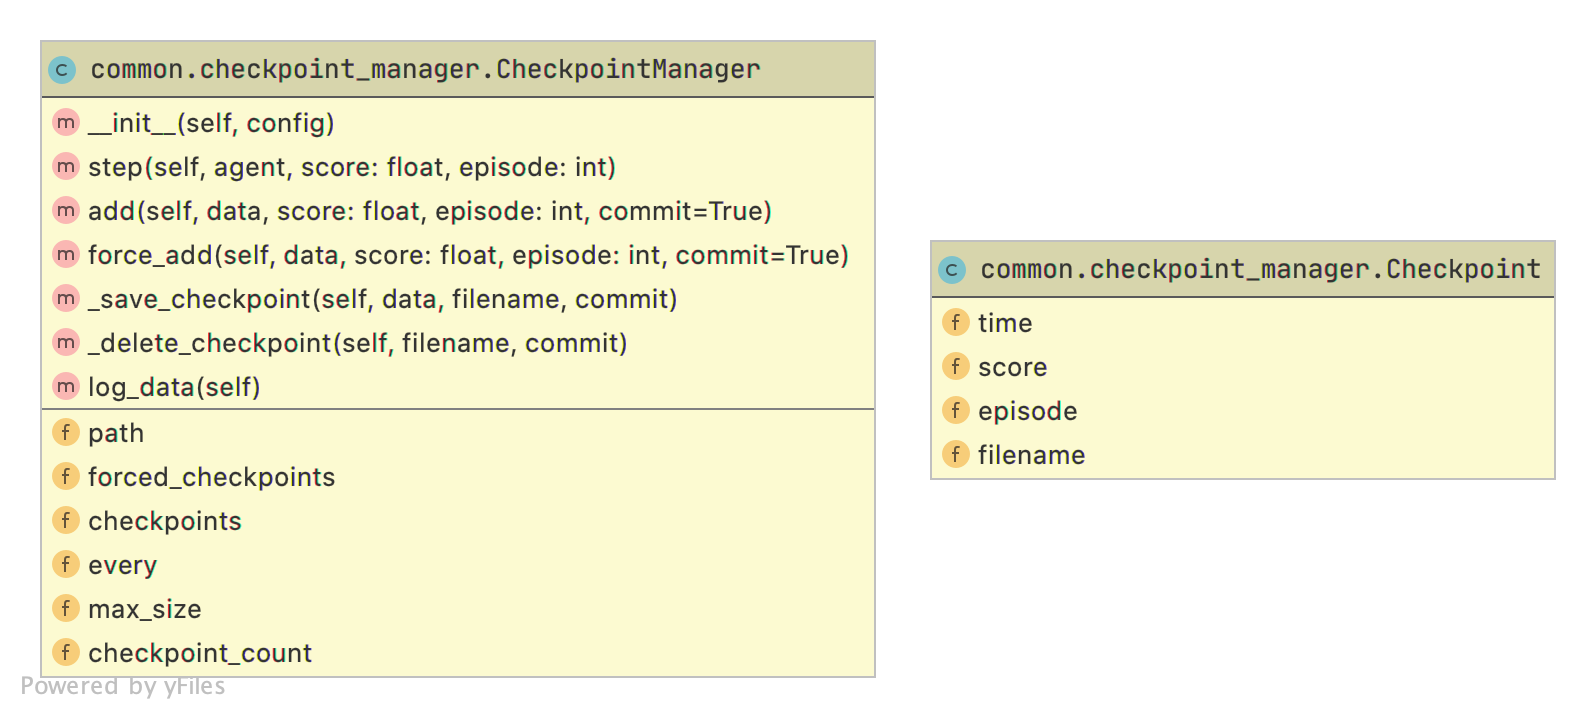
\includegraphics[width=0.7\textwidth]{app-checkpoint-manager.png}
    \caption{The class diagram of \texttt{CheckpointManager}, next to \texttt{Checkpoint}.}
    \label{fig:checkpoint-manager}
\end{figure}

\texttt{CheckpointManager} is a utility class whose purpose is to periodically capture snapshots of the agent model (the neural networks), along with other metadata (training epoch, hyperparameters, etc.) during training.
The best snapshots from training are used to reconstruct the agent and play the game in the evaluation environment.

Each snapshot file is several megabytes in size and a proper training session usually runs for hundreds of thousands (ideally, millions) of training steps.
In order to conserve disk space during training, the job of the checkpoint manager is to always compare the snapshots based on a predetermined metric in order to decide which ones to keep and which ones to remove.
The default metric used in this implementation is the average score over the last 100 episodes (an episode in the context of Pac-Man means a full level playthrough from board initialization until a terminal state is reached).

A separate \textbf{``forced'' checkpoint} is taken at the end of training, regardless of the score metric.
This is done because most algorithms don’t stabilize until the very end of training.
However, despite more reliably reaching good scores, well-performing agents do sometimes score lower than previous record high-scores induced by earlier local optima or by chance.

The manager is configurable -- its adjustable properties are the checkpoint frequency \texttt{every}, 
representing the number of steps between two consecutive snapshots, and the allowed capacity
\verb|max_size|, the maximum number of files it can store during a training run.

\subsection{Agent Modules} \label{section:agent-modules}

The framework contains a collection of agents, currently consisting of four different algorithms in the DQN family.
The relations among the agent classes is detailed in Figure \ref{fig:agent-class-diagram}.

\begin{figure}[h]
    \centering
    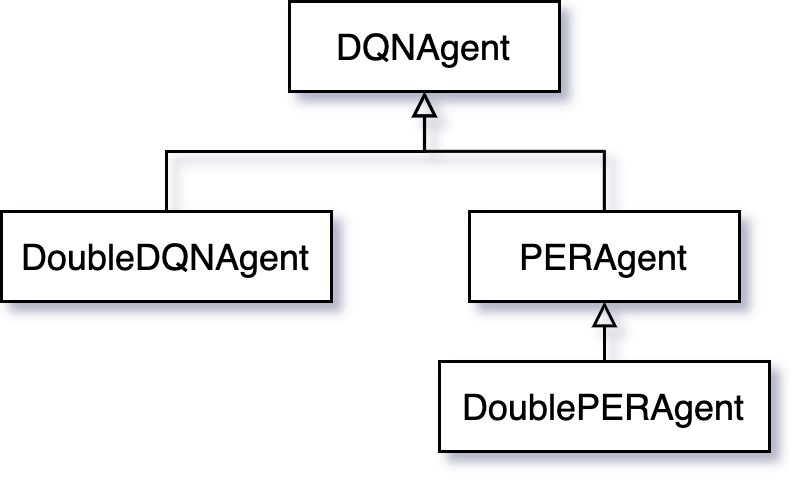
\includegraphics[width=0.5\textwidth]{app-agent-inheritance-diagram.png}
    \caption{A diagram representing the agent classes and their inheritance relations.}
    \label{fig:agent-class-diagram}
\end{figure}

\begin{figure}[h]
    \centering
    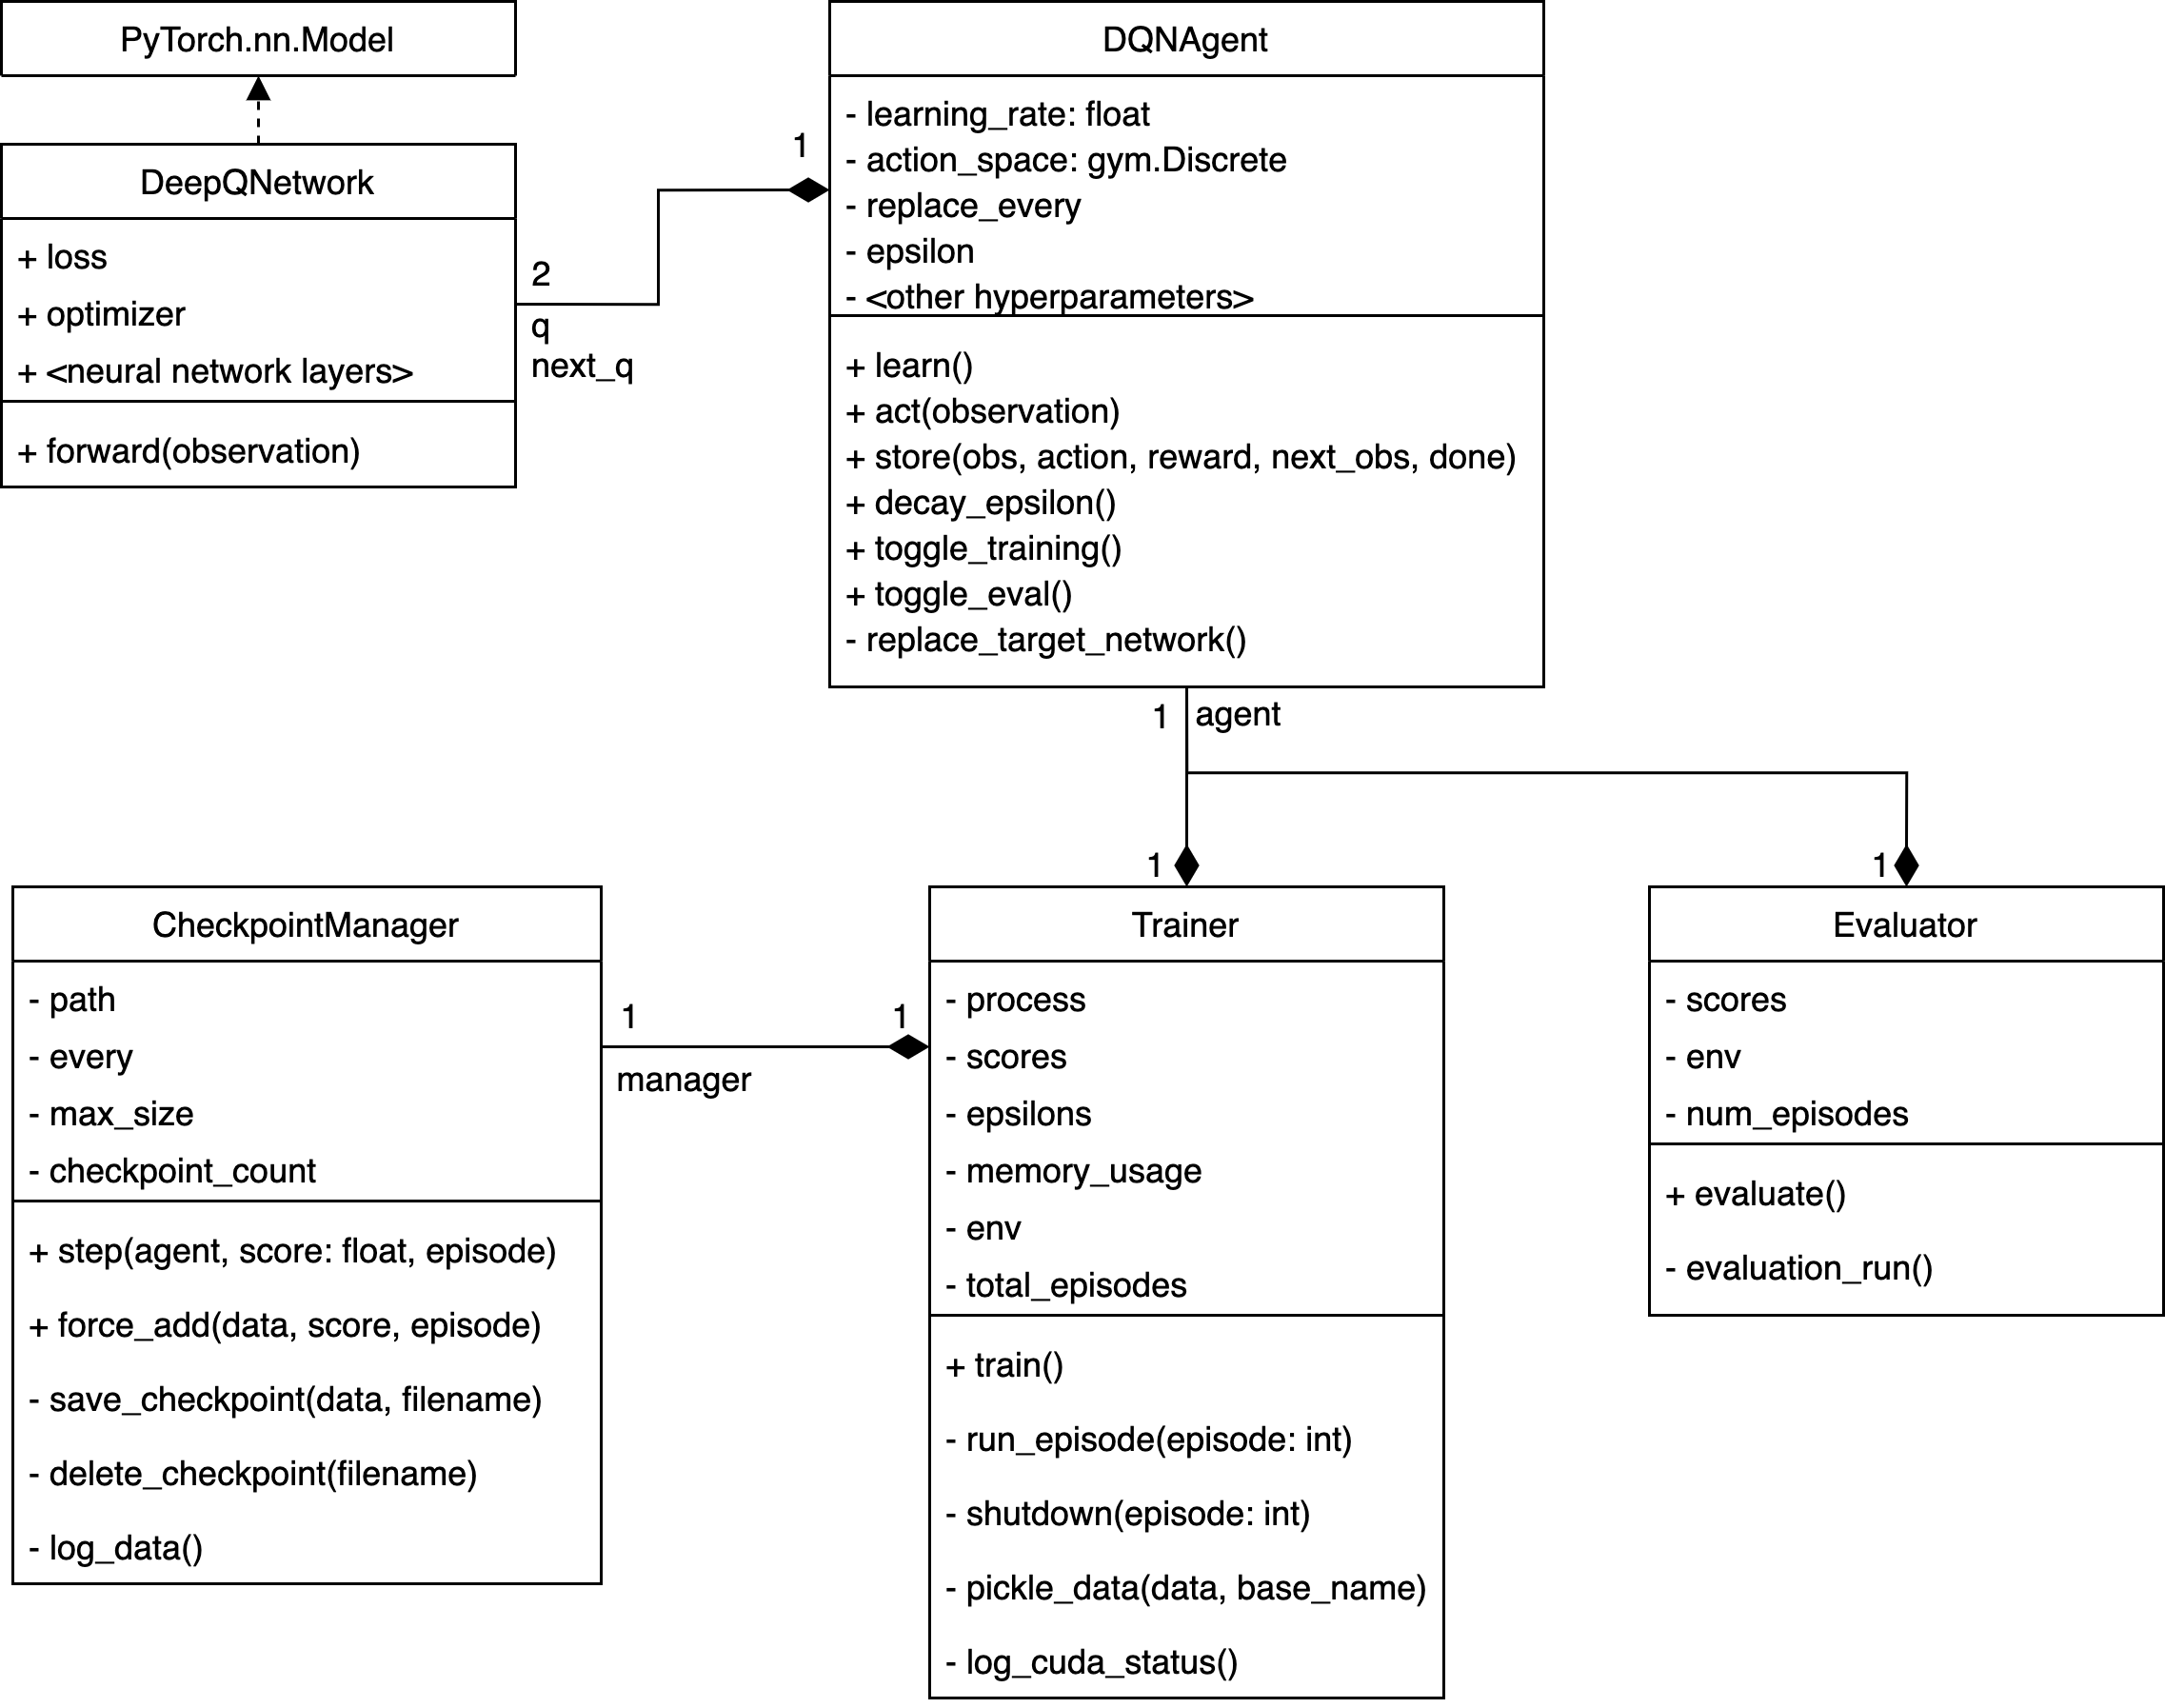
\includegraphics[width=\textwidth]{diagram_central_on_agent.png}
    \caption{A diagram representing how various classes interact with the \texttt{DQNAgent} class.
    The other agent classes follow the same blueprint.
    }
    \label{fig:agent-class-diagram}
\end{figure}

We will dissect the \texttt{deepq} package which, besides being a stand-alone implementation of the original DQN algorithm, represents the foundation upon which the other agents build upon.

The \texttt{deepq.Agent} module encapsulates the algorithm described in the DeepMind paper \cite{atari-dqn}.
An agent entity is initialized from a set of hyperparameters loaded from the configuration file in its \verb|__init__| method.

\begin{figure}
    \centering
    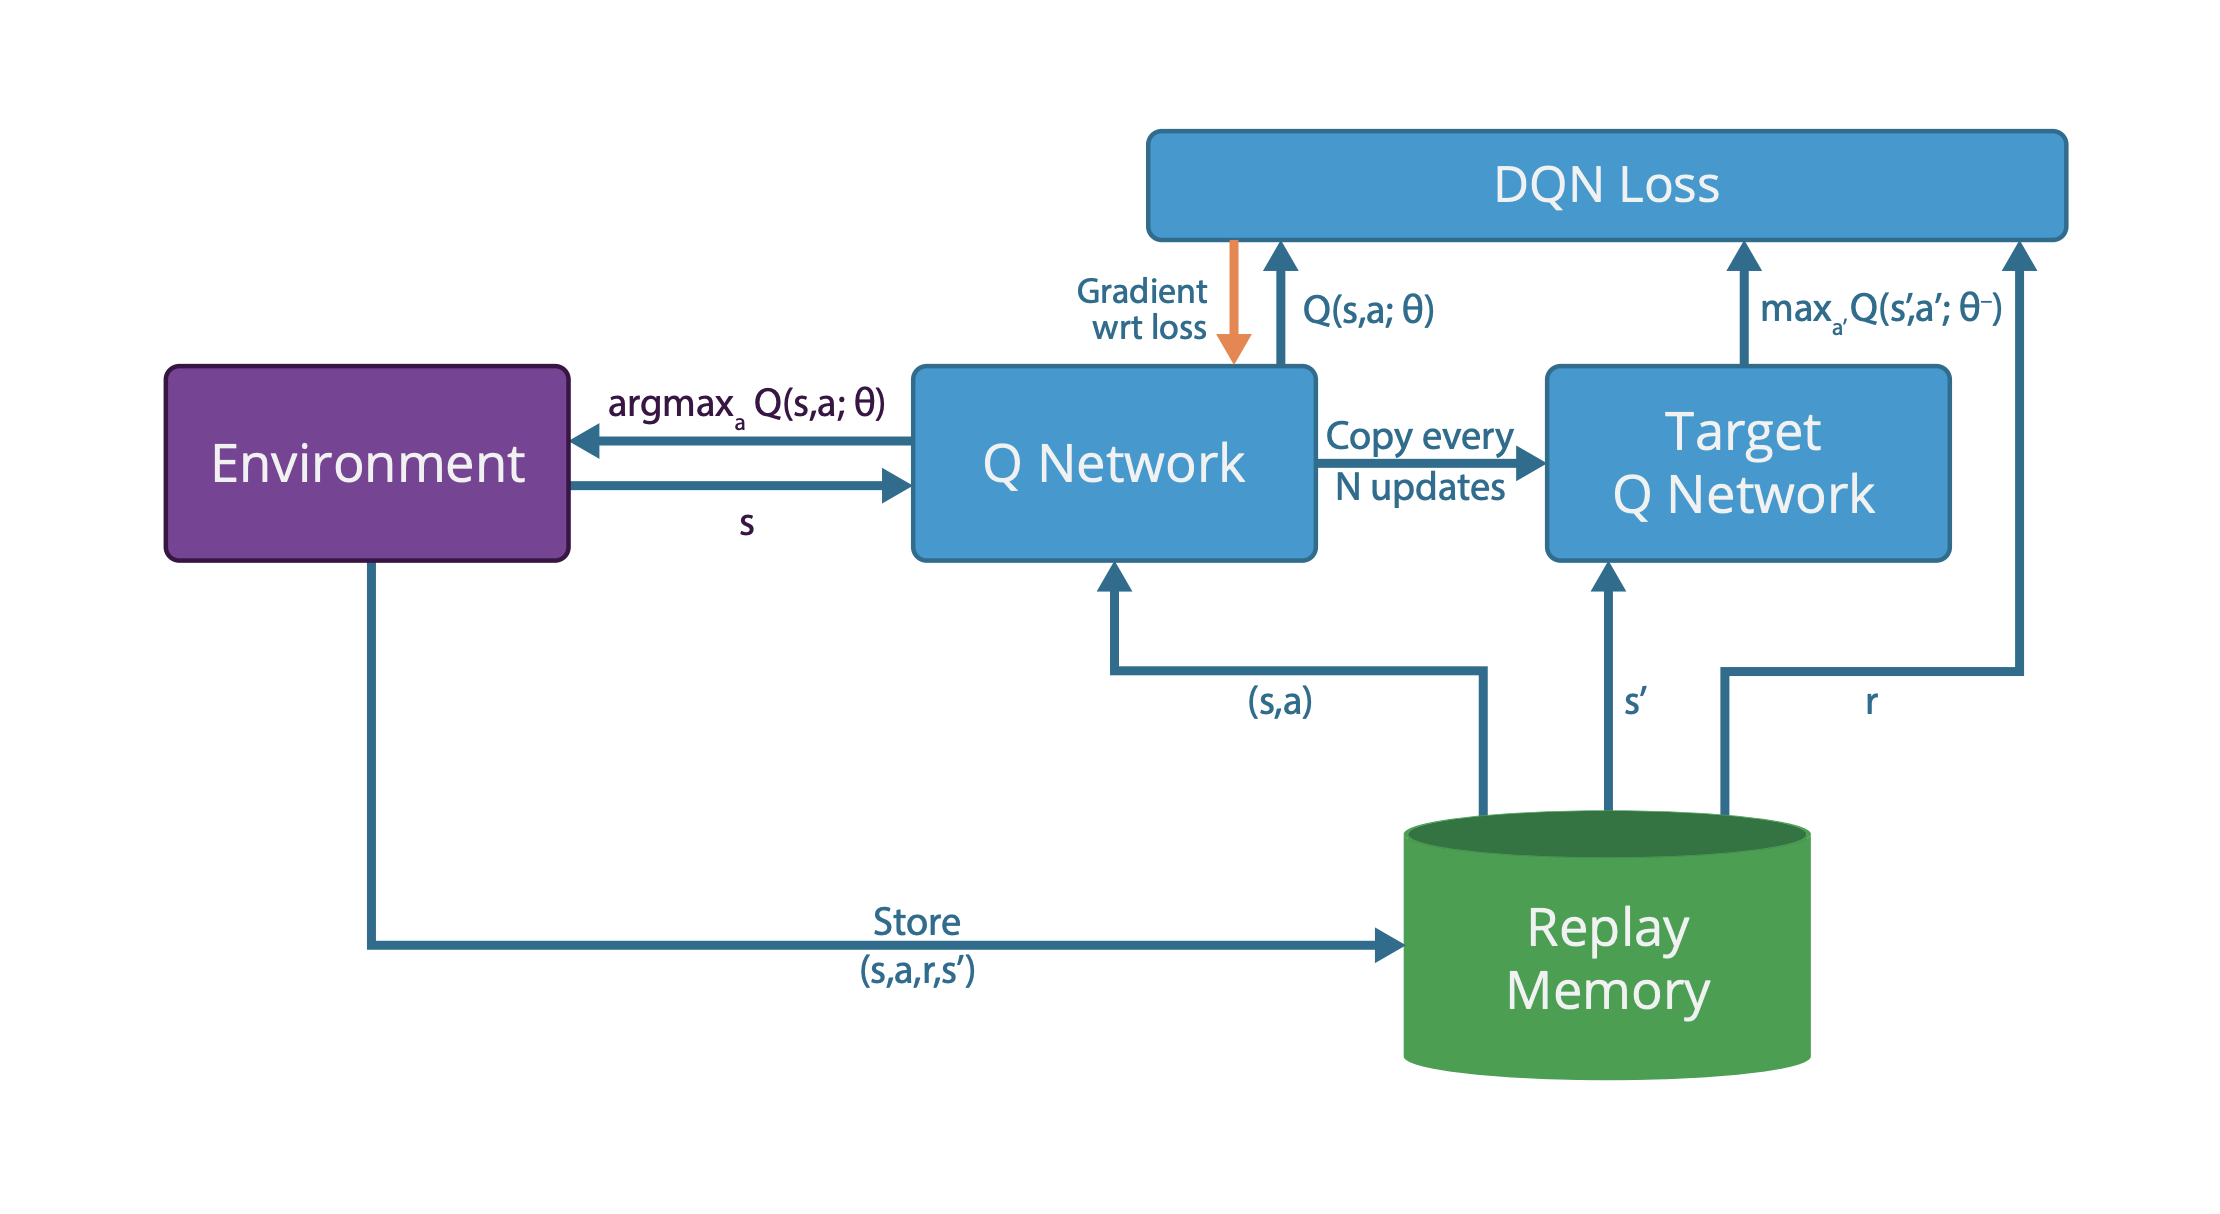
\includegraphics[width=0.9\textwidth]{dqn-architecture.png}
    \caption{High-level architectural view of an agent in classic DQN (Illustration from \cite{mpmdrl}).}
    \label{fig:dqn-architecture}
\end{figure}

The agent is fitted with two networks, which together constitute our model. We will explain in more depth in Subsection \ref{section:model-arch}. The networks are:
\begin{enumerate}
    \item the \textbf{main} Q-network, which provides the basis of action in the environment.
    \item the \textbf{target} Q-network, which estimates the Q-values of the next state.
\end{enumerate}

An agent class’s most central methods are \texttt{act} and \texttt{learn}.

The \texttt{act} method of the \texttt{DQNAgent} entity chooses an action based on an $\varepsilon$-greedy policy.
This essentially means that our agent has a probability $\varepsilon \in [0, 1]$ of choosing a random action.
During the course of our training, $\varepsilon$ will linearly decrease, until a certain point (e.g., we stop at a 5\% chance and keep it there for the rest of our training) -- this is called epsilon decay.

\textbf{Epsilon decay} is implemented by a secondary function in our module, called when a training episode finishes (see \verb|decay_epsilon|).
The process of decaying $\varepsilon$ is crucial to the convergence guarantees of most reinforcement learning algorithms.
It manages proper exploration of the environment.
Without proper control over this aspect, the agent can and will tend to get stuck in local optima.

The \verb|learn| method encapsulates the core of the system and runs one step of mini-batch gradient descent, as explained in Section \ref{section:dqn}.
The steps of the algorithm are broken down below.

Firstly, a mini-batch of transitions is sampled uniformly from our \textbf{replay memory}.
A transition represents a unit of agent experience and has the form $(s, a, r, s')$, where $a$ is an action in the action space, $r \in \mathbb{R}$ is the reward signal, $s$ is an observation (or state) of our agent and $s'$ is its successor state (observed after taking action $a$).

The Q-values are computed by a forward pass through our main network, for all states $s$ in our mini-batch, obtaining the main Q-value matrix.
This process can be accelerated, as the implementation is capable of leveraging GPU processing.
However, we are interested only in the actions $a$ which were taken during the actual play-through of our agent.
We reduce this matrix to a row vector, by only selecting the relevant action $a$ for every set of Q-values.

What in the original paper is denoted as $y_i$ will be computed by the agent in vector form by computing the mean-squared error function of the two vectors.
Using the computed loss, we take a step of mini-batch gradient descent.
Our optimizer is \verb|RMSProp|, as in the original work \cite{atari-dqn}.

Figure \ref{fig:dqn-architecture} provides a high-level recap, using a graphical depiction of how the different components interact during the learning step of the agent.

% \clearpage

\subsubsection{Model Architecture and the \texttt{DeepQNetwork} Class} \label{section:model-arch}

% Add a figure generated with https://github.com/ashishpatel26/Tools-to-Design-or-Visualize-Architecture-of-Neural-Network

Our model consists of two networks, the \textbf{main} and \textbf{target} deep Q-networks.
They are convolutional neural networks, sharing the same architecture.
A deep Q-network is composed of three layers: the first ConvNet layer applies a $8 \times 8$ filter with a stride of 4, the second ConvNet layer applies a $4 \times 4$ filter with a stride of 2, while the final layer is a fully-connected layer with 256 rectifier units \cite{atari-dqn}.
Both convolutional layers are followed by a rectifier nonliniarity.

The \textbf{input} to either network is a stack of $k$ frames, denoted conceptually as $s$ (or $s'$ in the case of the successor state, fed into the target network).
Stacking multiple frames captures the motion aspect of the game environment, which is essential for decision-making.
To reduce the storage space taken by the state representation, any frame captured from the emulator is transformed through gray-scaling, then cropped, to produce an 84 $\times$ 84 grayscale image \cite{atari-dqn}.
This transformation function is implemented as a wrapper around the emulator, in the \texttt{wrappers} package.

The \textbf{output} is a distribution over actions in the finite action space of the environment.
In the case of Pac-Man, the action space consists of four directions.
The available actions are specified by the Gym environment.
Other environments may provide actions for firing a weapon or activating an item.

The above network architecture is implemented in \texttt{deepq.DeepQNetwork} as an extension to PyTorch’s \texttt{nn.Model}.
\texttt{nn.Model} is an abstract class describing a node in a PyTorch computation graph, any extension of which needs to implement the \texttt{forward} and \texttt{backward} methods.
In the case of a neural network, they correspond to the forward pass and the backpropagation step respectively.

\subsection{The \texttt{replay\_memory} Package} \label{section:replay-memory-implementation}

% \begin{figure}[ht]
%     \centering
%     \begin{subfigure}[b]{0.5\textwidth}
%         \centering
%         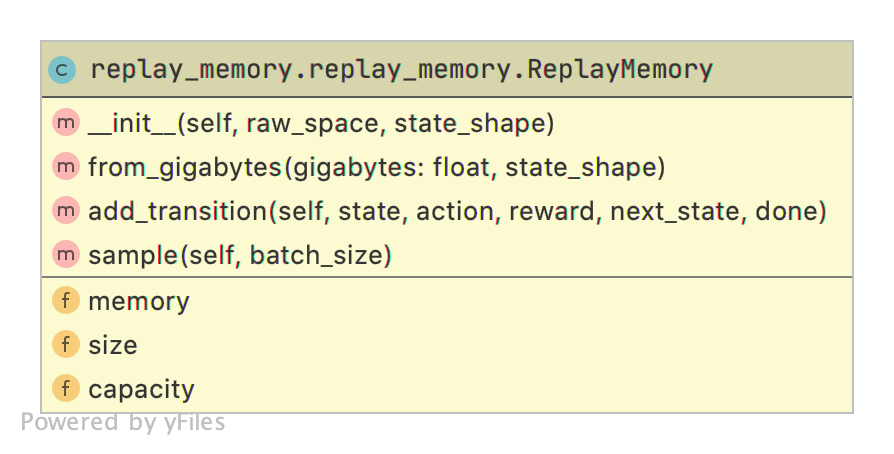
\includegraphics[width=0.5\textwidth]{app-replay-memory-class.png}
%         \caption{Class diagram of \texttt{ReplayMemory}.}
%         \label{fig:rm-diagram}
%     \end{subfigure}%
%     \hfill
%     \begin{subfigure}[b]{0.5\textwidth}
%         \centering
%         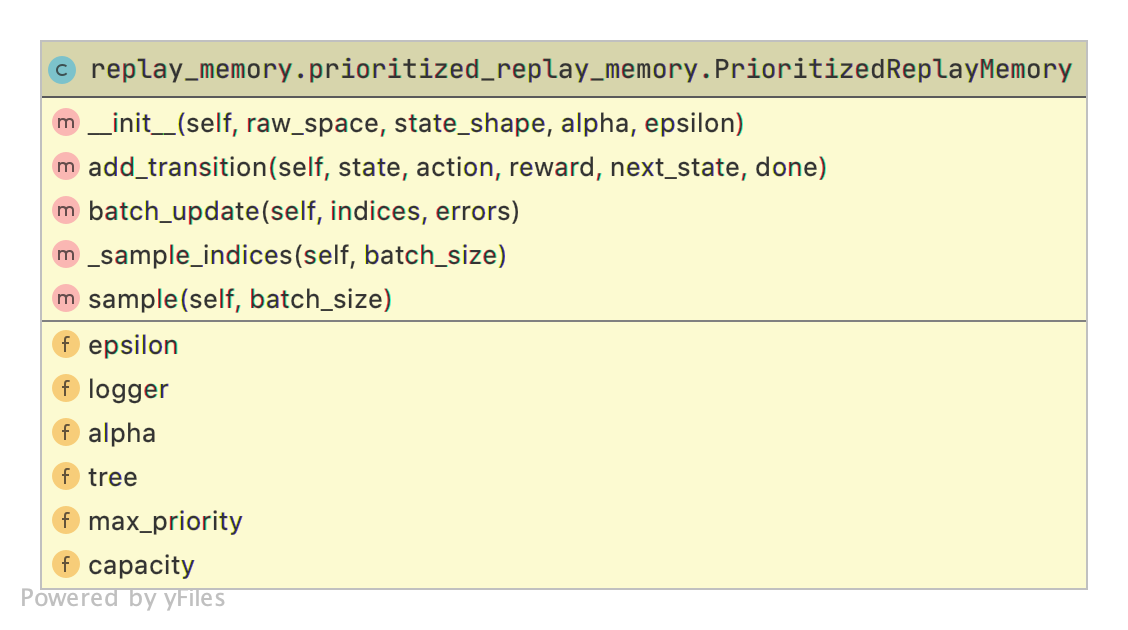
\includegraphics[width=0.5\textwidth]{app-prioritized-replay-memory-class.png}
%         \caption{\texttt{PrioritizedReplayMemory}}
%         \label{fig:prm-diagram}
%     \end{subfigure}
% \end{figure}
\begin{figure}[ht]
    \centering
    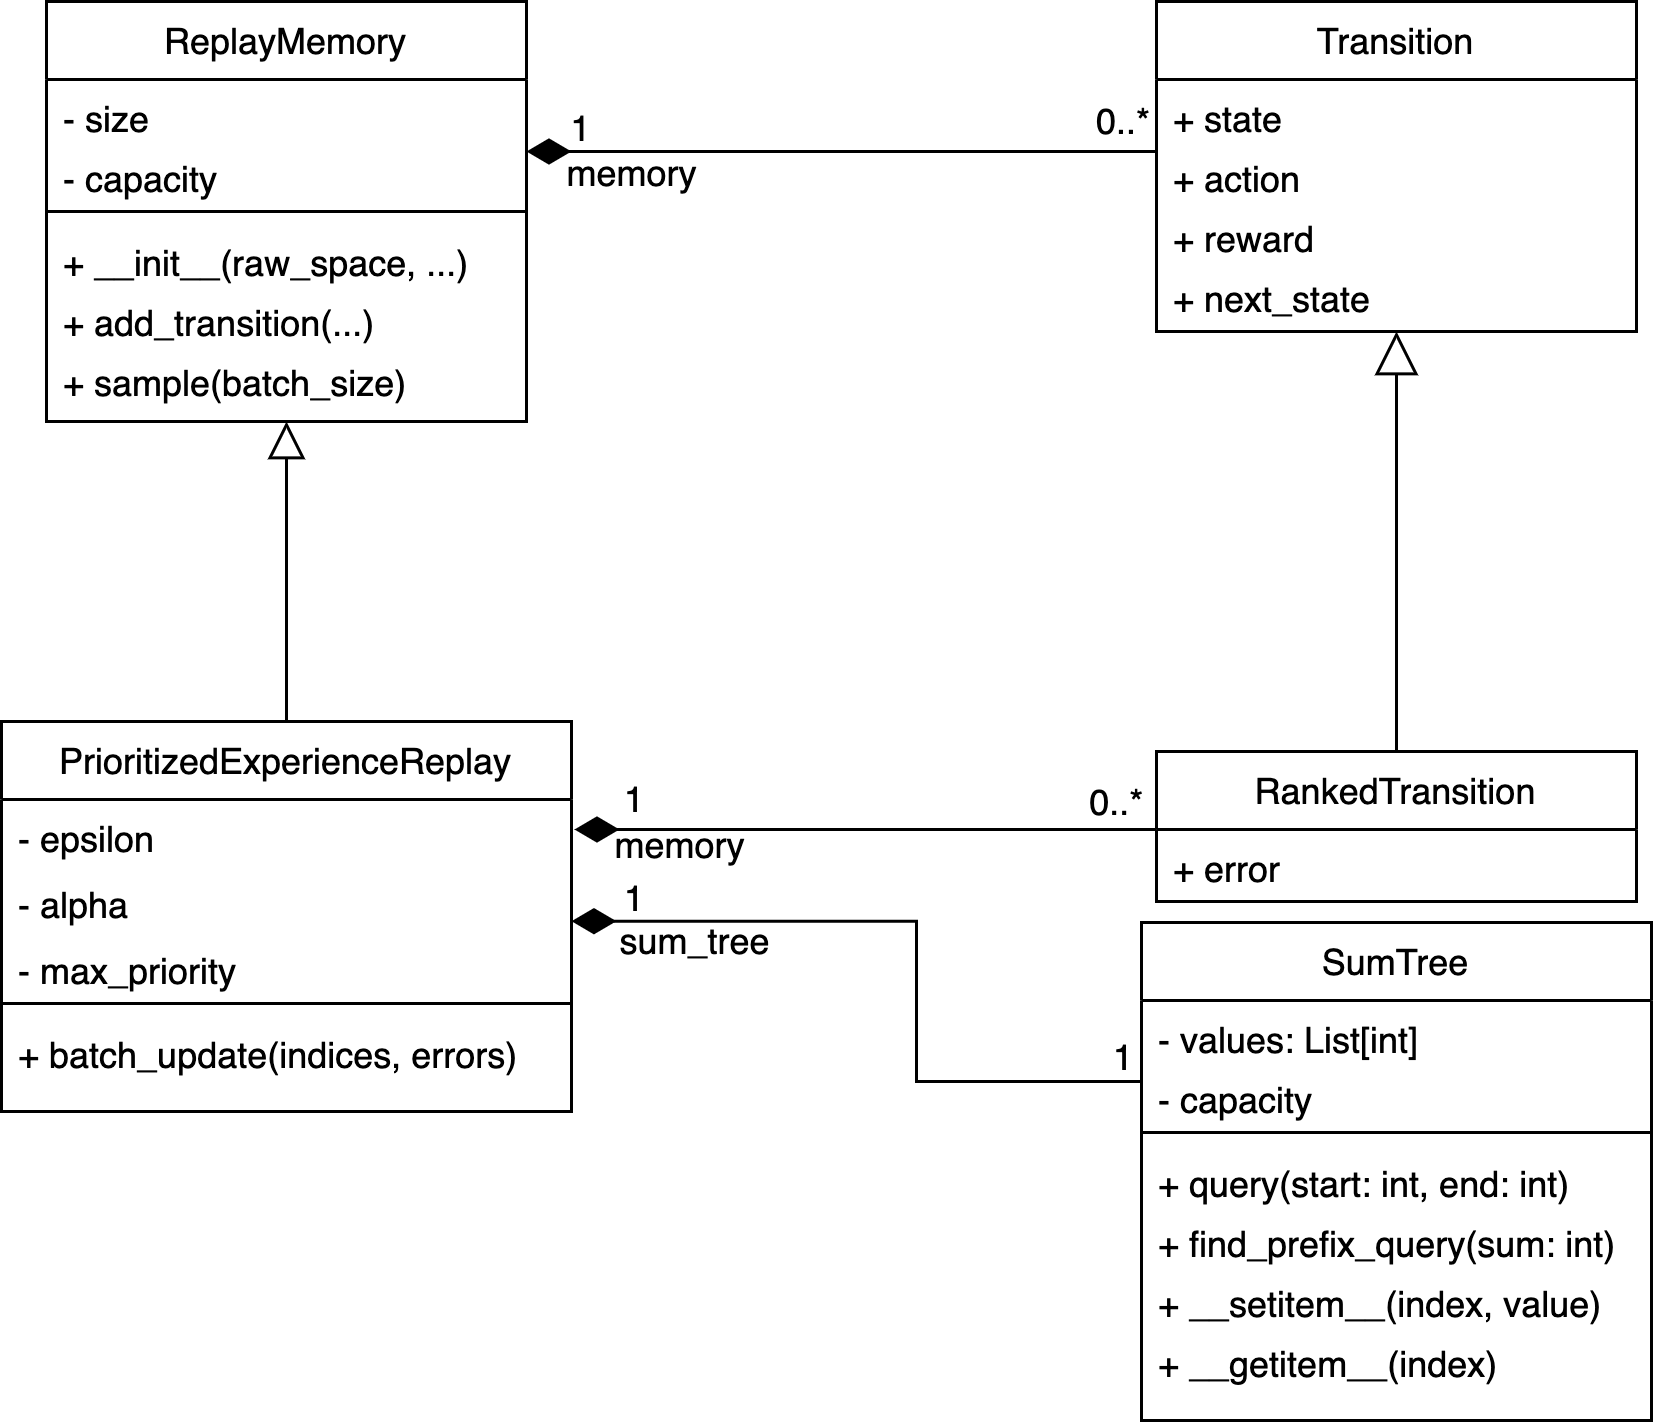
\includegraphics[width=\textwidth]{diagram_central_on_replay_memory.png}
    \caption{Diagram representing the \texttt{replay\_memory} classes and the relations among them.
    \texttt{SumTree} is also shown in this diagram due to its relevance to the functioning of the replay mechanism.}
\end{figure}

The project provides two implementations for the agent’s replay memory.

\texttt{ReplayMemory} provides a simple buffer from which we can sample experiences uniformly at random. This is used in DQN and in double Q-learning as well, as it does not impact the advantages of double learning.

\texttt{PrioritizedReplayMemory} is a more complex mechanism which memorizes the TD-errors of transitions and computes some priorities at every learning step, according to the algorithm in Section \ref{section:per}.
The prioritized sampling operation does not use a uniform distribution.
Instead, we use a sum tree to select transitions according to the error-based probability distribution.

Both implementations are able to deduce their maximum capacity from the total amount of memory (in gigabytes) given in the configuration file.
This mechanism is useful for remote execution on cloud instances, where as the amount of RAM available on the machine is pre-determined. We can specify a fixed chunk of memory to be allocated to the training process, to use as much of the available resources as possible.

\clearpage

\section{Technologies} \label{section:technologies}
Our framework leverages the stability of several battle-tested machine learning libraries.
Our choice of tools allows us to focus on the quality and performance of our implementation.
Our stack supports both CPU and GPU processing and allows quick prototyping, which was essential in the early stages of the project.
Below we present the most important libraries we use and mention their role in our project.
% possible extensions: Google Cloud Compute, TensorBoard, Anaconda, matplotlib

\subsection*{PyTorch}
\textbf{PyTorch} is an open-source machine learning library based on the Torch library.
It was created with a focus on the Python language \cite{pytorch-book} and thus has a strong interface for Python, although a C++ interface is also provided.
PyTorch has been built for speed and provides GPU-accelerated tensor support as well as a strong neural network package -- \verb|torch.nn|.
A distinguishable mechanic of this framework is its auto-differentiation implementation (called \texttt{autograd}) which allows building dynamic computation graphs, making the framework flexible and suitable for quickly prototyping machine learning models.
PyTorch is used in our framework to build the convolutional networks and to perform tensor computations, an integral part of our algorithm implementations.

\subsection*{NumPy}
NumPy is a scientific computing package for Python, supporting linear algebra, and featuring a complex random number library and versatile data structures for vectorized computation.
We use NumPy \verb|ndarray|s as a CPU-only equivalent to PyTorch's tensors, in areas of our program which do not need to support both modes of computation.
For example, the replay memory's buffer is exclusively held in main memory and thus does not require tensors, but we do perform vectorized operations and operations involving randomization.
Besides its speed (NumPy's core functionality is written in C), another important benefit is its comprehensive documentation.

\subsection*{OpenAI Gym}
In order to test our agent implementations, we rely on an excellent solution developed by the OpenAI team.
\textbf{OpenAI Gym} \cite{openai-gym} provides ready-made reinforcement learning environments, as well as flexible tools with which programmers can create their own.
We use OpenAI's supplied Atari environments, which provide interfaces to keep track of in-game score, lives, health or other indicators.
Those variables, primarily the score, serve as factors in the reward computation.

\subsection*{Jupyter Notebook}
Jupyter Notebook is a web-based environment for creating interactive ``notebooks'' -- documents which interleave Python code with Markdown notes, \texttt{matplotlib} plots and other objects.
They are a great tool for quickly prototyping models and documenting one's solution to a problem and are in widespread use in the Python data science community.
Juypter Notebook is only one project among many released by Project Jupyter as open-source software.
We extensively used notebooks for protyping during the early phase of the framework.
We incorporate a separate directory for special notebooks for studying algorithm performance, to plot agent performance and to compare different training runs.

\section{User Manual} \label{section:user-manual}
This section presents the basics of operating our framework to use one of our existing agents in the library to run a training job and collect its data.
Below we list commands for training, evaluation and deployment and we explain flags and configuration variables.

\subsection*{Training}
Training can be initialized locally, on the user's computer, or remotely, in a cloud environment.
The starting script \verb|train.py| initializes the \verb|Trainer|, changes its mode of operation based on the relevant flags and loads the configuration file.
\begin{verbatim}
python train.py -c <configuration-file> <options>
\end{verbatim}

This is an example of a \verb|YAML| configuration file, written for the DQN algorithm:
\begin{verbatim}
training:
  name: dqn
  ...
model:
  learning_rate: 1e-4
  gamma: 0.99
  ...
checkpoints:
  path: ../data/checkpoints/
  max_size: 5
  every: 500
logs:
  path: ../data/logs/
monitor:
  path: ../data/monitor/
evaluation:
  num_episodes: 200
  ...
\end{verbatim}

The \verb|training| node contains general information about the training job, including a label to track it when comparing multiple results.

The \verb|model| node contains hyperparameters required by a particular algorithm to run.
A lot of the parameters are common among the various implementations (for example, \verb|learning_rate| is a general parameter of the neural network).

The \verb|checkpoints| settings group controls the checkpoint manager, as discussed in its relevant subsection in the \emph{Implementation} section.

\verb|monitor| and \verb|evaluation| control the \textbf{evalutation}. Those are not relevant to the training per se, but sometimes we want to associate the evaluation settings to the algorithm itself, so we can put them into the same file, instead of having two separate configurations (although using separate configurations between traning and evaluation is possible).

Before the launch of the training job, the user can specify the desired algorithm using two special flags.
\verb|--per| trains the agent using prioritized experience replay.
\verb|--doubledqn| train the agent using double Q-learning.
Combining these flags in whichever order will enable both approaches simultaniously by loading and training the \verb|DoublePERAgent|.

\subsection*{Evaluation}
For evaluation, we similarly run:
\begin{verbatim}
    python play.py -c <configuration-file> <options>
\end{verbatim}

The evaluation environment is designed to test an agent in a more stable environment, with no randomization.
This running mode has the addition of outputing \textbf{video captures} of the emulator in a dedicated \verb|monitor| directory (as specified by the \verb|monitor.path| setting in the configuration), so that we can study an agent's behaviour by directly observing any strategies it might have developed or any areas in which it have failed to develop one.

\subsection*{Utility Scripts}
The \verb|data| directory stores the data associated to the training job, including logs, scores and checkpoints.
At the end of training, this directory is compressed into a \verb|results| file (using the \verb|gzip| standard) so the data directory itself is redundant and needs to be cleaned.
For this purpose, we provide a \verb|cleanup.sh| Bash script, for $*$nix systems, which removes the training files and re-initializes the required directory structure.

Additionally, we might want to make modifications to the implementation and want to keep the Python codebase compliant to PEP norms.
For this purpose we use the \verb|black| code formatter and the \verb|docformatter| utility for docstrings.
We provide a \verb|format.py| Python script, which combines those two and runs them recursively over every directory in our codebase, in order to keep everything tidy and uniformly stylized.

% might add TensorBoard usage
